% vim: set textwidth=78 autoindent:

\section{Creare applicazioni PyQGIS}

% when the revision of a section has been finalized, 
% comment out the following line:
% \updatedisclaimer

Uno degli obiettivi di QGIS è fornire non soltanto un'applicazione ma anche un set di librerie che possano essere usate per creare nuove applicazioni. Questo obiettivo è stato realizzato mediante la ristrutturazione delle libreria che ha avuto luogo dopo il rilascio della versione 0.8. Dal rilascio della versione 0.9, è possibile lo sviluppo di applicazioni indipendenti usando C++ o Python. Si raccomanda di usare QGIS 1.0.0 o superiore come base per le proprie applicazioni python poichè da questa versione si fornisce un API stabile e coerente.

In questo capitolo si darà un'occhiata al processo di creazione di un'applicazione Python indipendente. Il blog di QGIS ha vari esempi su come creare applicazioni PyQGIS\footnote{Un'applicazione creata usando Python ed i legami QGIS}. Useremo una di esse come punto di partenza per un'occhiata a come creare un'applicazione.

Le funzioni che vogliamo nell'applicazione sono:

\begin{itemize}
\item Caricare un layer vettoriale
\item Panoramica
\item Ingrandimento e riduzione
\item Ingrandimento alla completa estensione del layer
\item Impostazione di colori personalizzati al caricamento del layer
\end{itemize} 

Questo è un set di funzioni piuttosto minimo. Cominciamo progettando l'interfaccia grafica (GUI) usando Qt Designer.

\subsection{Progettare l'interfaccia grafica (GUI)}

Dato che stiamo creando un'applicazione minimale, useremo lo stesso approccio per l'interfaccia grafica. Usando Qt Designer, si crea una semplice finestra principale (MainWindow) priva di menu e barre degli strumenti. Questo ci da una lavagna bianca per lavorare. Per creare la finestra principale:

\begin{enumerate}
\item Creare una directory per sviluppare l'applicazione ed entrarci
\item Lanciare Qt Designer
\item Dovrebbe apparire la finestra di dialogo \qtdialog{New form}. Se non appare, scegliere
\qtdropmenuopt{New form...} dal menu \qtmainmenuopt{File}.
\item Scegliere \qtdropmenuopt{Main Window} dalla lista 
the \qtdropmenuopt{templates/forms} 
\item Premere \qtdropmenuopt{Create} 
\item Ridimensionare la nuova finestra ad una dimensione maneggevole
\item Trovare nella lista il widget \qtdropmenuopt{Frame} 
(sotto \qtdropmenuopt{Containers}) e trascinarlo nella finestra principale appena creata
\item Premere all'esterno della cornice per selezionare l'area della finestra principale 
\item Premere lo strumento \qtdropmenuopt{Lay Out in a Grid}. Quando si fa questo, ia cornice si allarga a riempire l'intera finestra principale
\item Salvare il modulo come \usertext{mainwindow.ui} 
\item \qtdropmenuopt{Exit} Qt Designer
\end{enumerate} 

Ora compilare il modulo usando l'interfaccia compilatore PyQt:

\begin{verbatim}
   pyuic4 -o mainwindow_ui.py mainwindow.ui
\end{verbatim}

Questo crea la sorgente Python per la finestra principale GUI. Poi si deve creare il codice dell'applicazione per riempire la lavagna bianca con alcuni strumenti che si possono usare.

\subsection{Creare la Finestra Principale}

Adesso siamo pronti a scrivere la classe \classname{MainWindow} che farà il vero lavoro.
Dato che ci vogliono parecchie linee, ci daremo un'occhiata a pezzi, cominciando con la sezione importazione e le impostazioni dell'ambiente:

\begin{verbatim}
1 # Loosely based on:
2 #   Original C++ Tutorial 2 by Tim Sutton
3 #   ported to Python by Martin Dobias
4 #   with enhancements by Gary Sherman for FOSS4G2007
5 # Licensed under the terms of GNU GPL 2
6
7 from PyQt4.QtCore import *
8 from PyQt4.QtGui import *
9 from qgis.core import *
10 from qgis.gui import *
11 import sys
12 import os
13 # Import our GUI
14 from mainwindow_ui import Ui_MainWindow
15 
16 # Environment variable QGISHOME must be set to the 1.0 install directory
17 # before running this application
18 qgis_prefix = os.getenv("QGISHOME")
\end{verbatim}

Un po' di questo dovrebbe apparire familiare dal nostro plugin, specialmente le importazioni PyQt4 e
QGIS. Alcune cose specifiche da notare sono le importazioni della nostra GUI alla linea
14 e l'importazione nella libreria CORE alla linea 9.

La nostra applicazione necessita di sapere dove trovare l'installazione di QGIS. Per questo, impostiamo l'ambiente variabile \usertext{QGISHOME} in modo che indichi la directory di installazione di QGIS 1.x Alla linea 20 memorizziamo questo valore dall'ambiente per un uso successivo.

Poi è necessario creare la nostra classe \classname{MainWindow} che conterrà tutta la logica della nostra applicazione.
\begin{verbatim}
21 class MainWindow(QMainWindow, Ui_MainWindow):
22 
23   def __init__(self):
24     QMainWindow.__init__(self)
25 
26     # Required by Qt4 to initialize the UI
27     self.setupUi(self)
28 
29     # Set the title for the app
30     self.setWindowTitle("QGIS Demo App")
31 
32     # Create the map canvas
33     self.canvas = QgsMapCanvas()
34     # Set the background color to light blue something
35     self.canvas.setCanvasColor(QColor(200,200,255))
36     self.canvas.enableAntiAliasing(True)
37     self.canvas.useQImageToRender(False)
38     self.canvas.show()
39 
40     # Lay our widgets out in the main window using a 
41     # vertical box layout
42     self.layout = QVBoxLayout(self.frame)
43     self.layout.addWidget(self.canvas)
44 
45     # Create the actions for our tools and connect each to the appropriate
46     # method
47     self.actionAddLayer = QAction(QIcon("(qgis_prefix + "/share/qgis/themes/classic/mActionAddLayer.png"),
48     \
49         "Add Layer", self.frame)
50     self.connect(self.actionAddLayer, SIGNAL("activated()"), self.addLayer)
51     self.actionZoomIn = QAction(QIcon("(qgis_prefix + "/share/qgis/themes/classic/mActionZoomIn.png"), \
52         "Zoom In", self.frame)
53     self.connect(self.actionZoomIn, SIGNAL("activated()"), self.zoomIn)
54     self.actionZoomOut = QAction(QIcon("(qgis_prefix + "/share/qgis/themes/classic/mActionZoomOut.png"), \
55         "Zoom Out", self.frame)
56     self.connect(self.actionZoomOut, SIGNAL("activated()"), self.zoomOut)
57     self.actionPan = QAction(QIcon("(qgis_prefix + "/share/qgis/themes/classic/mActionPan.png"), \
58         "Pan", self.frame)
59     self.connect(self.actionPan, SIGNAL("activated()"), self.pan)
60     self.actionZoomFull = QAction(QIcon("(qgis_prefix + "/share/qgis/themes/classic/mActionZoomFullExtent.png"), \
61         "Zoom Full Extent", self.frame)
62     self.connect(self.actionZoomFull, SIGNAL("activated()"),
63     self.zoomFull)
64 
65     # Create a toolbar
66     self.toolbar = self.addToolBar("Map")
67     # Add the actions to the toolbar
68     self.toolbar.addAction(self.actionAddLayer)
69     self.toolbar.addAction(self.actionZoomIn)
70     self.toolbar.addAction(self.actionZoomOut);
71     self.toolbar.addAction(self.actionPan);
72     self.toolbar.addAction(self.actionZoomFull);
73 
74     # Create the map tools
75     self.toolPan = QgsMapToolPan(self.canvas)
76     self.toolZoomIn = QgsMapToolZoom(self.canvas, False) # false = in
77     self.toolZoomOut = QgsMapToolZoom(self.canvas, True) # true = out
\end{verbatim}

Le linee da 21 a 27 costituiscono la dichiarazione di base e l'inizializzazione della 
\classname{MainWindow} e le impostazioni dell'interfaccia utente usando il metodo 
\method{setupUi}. Questo è richiesto per tutte le applicazioni.

Quindi si imposta il titolo per l'applicazione così dice qualcosa di più interessante che \usertext{MainWindow} (linea 30). Una volta che questo è fatto, siamo pronti a completare l'interfaccia utente. Quando la si è creata in Designer, l'abbiamo lasciata abbozzata---solo una finestra principale e una cornice. Si può aver aggiunto un menu ed una barra degli strumenti usando Designer, comunque lo faremo con Python.

Nelle linee 33 fino a 38 si impostano il canvas della mappa, il colore di sfondo a celeste e si abilita la distorsione minima. Si specifica anche di non usare una \classname{QImage} per la rappresentazione grafica (fidatevi a questo riguardo) e poi si imposta il canvas a visibile chiamando il metodo \method{show}.

Quindi si imposta il layer affinchè usi uno schema a riquadro verticale all'interno della cornice e si aggiunge ad esso il canvas della mappa alla linea 43.

Le linee da 48 a 63 impostano le azioni e le connessioni per gli strumenti nella nostra barra degli strumenti. Per ogni strumento, si crea una \classname{QAction} usando l'icona che abbiamo definito nel tema classico di QGIS. Poi colleghiamo il segnale \usertext{activated} dallo strumento al metodo nella nostra classe che gestirà l'azione. Questo è simile a come impostare le cose nell'esempio plugin.

Una volta che si hanno l'azione e la connessione, si deve aggiungerle alla barra degli strumenti.
Nelle linee da 66 a 72 si crea la barra degli strumenti e si aggiunge ad esse ogni strumento.

Infine si creano tre strumenti mappa per l'applicazione (linee da 75 a
77). Si useranno gli strumenti mappa in un momento dopo aver definito i metodi per rendere l'applicazione funzionale. Vediamo i metodi per gli strumenti mappa.

\begin{verbatim}
78   # Set the map tool to zoom in
79   def zoomIn(self):
80     self.canvas.setMapTool(self.toolZoomIn)
81 
82   # Set the map tool to zoom out
83   def zoomOut(self):
84     self.canvas.setMapTool(self.toolZoomOut)
85 
86   # Set the map tool to 
87   def pan(self):
88    self.canvas.setMapTool(self.toolPan)
89 
90   # Zoom to full extent of layer
91   def zoomFull(self):
92     self.canvas.zoomFullExtent()
\end{verbatim}

Per ogni strumento della mappa, è necessario un metodo che corrisponde alla connessione fatta per ogni azione. Nelle linee da 79 a 88 impostiamo un metodo per ognuno dei tre strumenti che interagiscono con la mappa. Quando uno strumento è attivato premendo il suo pulsante nella barra degli strumenti, è attivato il metodo corrispondente che "dice" al canvas della mappa che quello è lo strumento attivo. Lo strumento attivo governa cosa avviene quando il mouse è premuto nel canvas.

Lo strumento \usertext{zoom to full extent} non è uno strumento mappa---svolge il suo lavoro senza richiedere un  click sulla mappa. Quando è attivato, viene chiamato il metodo del canvas della mappa
\method{zoomFullExtent} (line 92).  Questo completa l'implementazione di tutti i nostri strumenti eccetto uno: lo strumento \usertext{Add Layer}. %FIXME 
Analizziamolo:


\begin{verbatim}
93   # Add an OGR layer to the map
94   def addLayer(self):
95     file = QFileDialog.getOpenFileName(self, "Open Shapefile", ".", "Shapefiles
96     (*.shp)")
97     fileInfo = QFileInfo(file)
98 
99     # Add the layer
100     layer = QgsVectorLayer(file, fileInfo.fileName(), "ogr")
101
102    if not layer.isValid():
103      return
104
105    # Change the color of the layer to gray
106    symbols = layer.renderer().symbols()
107    symbol = symbols[0]
108    symbol.setFillColor(QColor.fromRgb(192,192,192))
109
110    # Add layer to the registry
111    QgsMapLayerRegistry.instance().addMapLayer(layer);
112
113    # Set extent to the extent of our layer
114    self.canvas.setExtent(layer.extent())
115
116    # Set up the map canvas layer set
117    cl = QgsMapCanvasLayer(layer)
118    layers = [cl]
119    self.canvas.setLayerSet(layers)
\end{verbatim}

Nel metodo \method{addLayer} si usa \classname{QFileDialog} per trovare il nome del file da caricare. Questo è fatto alla linea 96. Va notato che si specifica un "filtro" così la finestra di dialogo mostrerà solamente file di tipo \filename{.shp}.

Di seguito nella 97 si crea un oggetto \classname{QFileInfo} dal percorso del file shape.  Ora il layer è pronto per essere creato nella linea 100. Usando l'oggetto \classname{QFileInfo} per arrivare al file dal percorso abbiamo specificato il nome del layer quando esso viene creato.  Per essere sicuri che il layer sia valido e non causi alcun problem quando caricato, controlliamolo nella linea 102. Se non va bene, lo abbandoniamo e non lo aggiungiamo al canvas della mappa.

Normalmente i layer sono aggiunti con un colore random. Ora si vogliono modificare i colori del layer per rendere la vista più piacevole. Inoltre sappiamo che si deve aggiungere il layer \filename{world\_borders} alla mappa e questo lo renderà più bello sul nostro sfondo blu. Per cambiare il colore, è necessario prendere il simbolo usato per la rappresentazione grafica e usarlo per impostare un nuovo colore di riempimento. Questo è fatto dalla linea 106 alla 108. 

Tutto ciò che rimane ora è aggiungere il layer al registro e alcune altre voci di manutenzione (linee da 111 a 119). Questa roba è standard nell'aggiungere un layer ed il risultato finale sono i bordi del mondo su uno sfondo celeste. La sola cosa che si potrebbe non voler impostare è l'estensione del layer, se si deve aggiunge più di un layer nell'applicazione.

Questo è il cuore dell'applicazione e completa la classe \classname{MainWindow}. 

\subsection{Conclusione}

Il resto del codice scritto sotto crea l'oggetto \object{QgsApplication}, imposta il percorso all'installazione di QGIS, imposta il metodo \method{main} e infine avvia l'applicazione. L'unica altra cosa da notare è che noi muoviamo la finestra dell'applicazione all'angolo superiore sinistro dello schermo. Potremmo anche essere fantasiosi e usare il Qt API per centrarla sullo schermo.

\begin{verbatim}
120 def main(argv):
121   # create Qt application
122   app = QApplication(argv)
123 
124   # Initialize qgis libraries
125   QgsApplication.setPrefixPath(qgis_prefix, True)
126   QgsApplication.initQgis()
127 
128   # create main window
129   wnd = MainWindow()
130   # Move the app window to upper left
131   wnd.move(100,100)
132   wnd.show()
133 
134   # run!
135   retval = app.exec_()
136   
137   # exit
138   QgsApplication.exitQgis()
139   sys.exit(retval)
140 
141 
142 if __name__ == "__main__":
143   main(sys.argv)
\end{verbatim}

\subsection{Lanciare l'applicazione}

Ora si può lanciare l'applicazione e vedere cosa succede. Se si è come molti sviluppatori, probabilmente la si è testata man mano che la si scriveva. 

Prima di lanciare l'applicazione, si devono impostare alcune variabli d'ambiente. 

\nix{}\osx{}
\begin{verbatim}
export LD_LIBRARY_PATH=$HOME/qgis/lib%$
export PYTHONPATH=$HOME/qgis/share/qgis/python
export QGISHOME=$HOME/qgis%$
\end{verbatim}

\win{}
\begin{verbatim}
set PATH=C:\qgis;%PATH%
set PYTHONPATH=C:\qgis\python
set QGISHOME=C:\qgis
\end{verbatim}

Si assume che
\begin{itemize}
\item\nix{}\osx{}QGIS sia installato nella home directory in 
\filename{qgis}. 
\item\win{}QGIS sia installato in \filename{C:\textbackslash qgis}.
\end{itemize}

All'avvio l'applicazione appare così:

%\begin{figure}[ht]
%\begin{center}
%  \caption{Starting the new demo application}\label{fig:demo_app_startup}%\smallskip
%  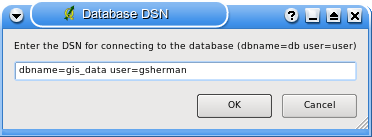
\includegraphics[scale=0.8]{getdsn}
%\end{center}
%\end{figure}

Per aggiunger il layer \filename{world\_borders}, premere lo strumento 
\usertext{Add Layer} e navigare alla directory dei dati.
Selezionare lo shapefile e premere \button{Open} per aggiungerlo alla mappa. 
Il nostro colore di riempimento personalizzato è aggiunto e il risultato è:

%\begin{figure}[ht]
%\begin{center}
%  \caption{Adding a layer the demo application}\label{fig:demo_app_done}%\smallskip
%  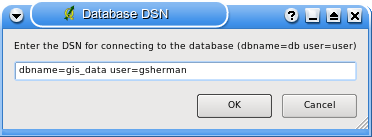
\includegraphics[scale=0.8]{getdsn}
%\end{center}
%\end{figure}

Creare un'applicazione PyQGIS è veramente molto facile. In meno di 150 linee di codice avrete un'applicazione che può caricare uno shapefile e navigare la mappa. Se giocate un po' con la mappa, noterete che funzionano anche alcune delle caratteristiche integrate del canvas, incluso lo scorrimento con il mouse e lo spostamento della vista premendo la barra spaziatrice \keystroke{Space} contemporaneamente al mouse.

Diverse applicazioni sofisticate sono state create con PyQGIS e molte altre sono in lavorazione. Questo è impressionante, se si considera che questo sviluppo è avvenuto anche prima del rilascio ufficiale di QGIS 1.0.

\begin{Tip}\caption{\textsc{Documentazione per PyQGIS}}
\qgistip{Se state scrivendo un plugin o un'applicazione PyQGIS, avrete bisogno di far riferimento alle documentazioni QGIS API (\url{http://doc.qgis.org}) e alla Guida di riferimento di PyQt Python
(\url{http://www.riverbankcomputing.com/Docs/PyQt4/pyqt4ref.html}). Questi documenti forniscono informazioni sulle classi e sui metodi che saranno usati per portare la vostra creazione in Python alla vita.
}
\end{Tip} 
